\section{Detecting a Single Object}
\begin{frame}{}
    \LARGE Object Detection: \textbf{Detecting a Single Object}
\end{frame}

\begin{frame}[allowframebreaks]{Detecting a Single Object}
    \begin{figure}
        \centering
        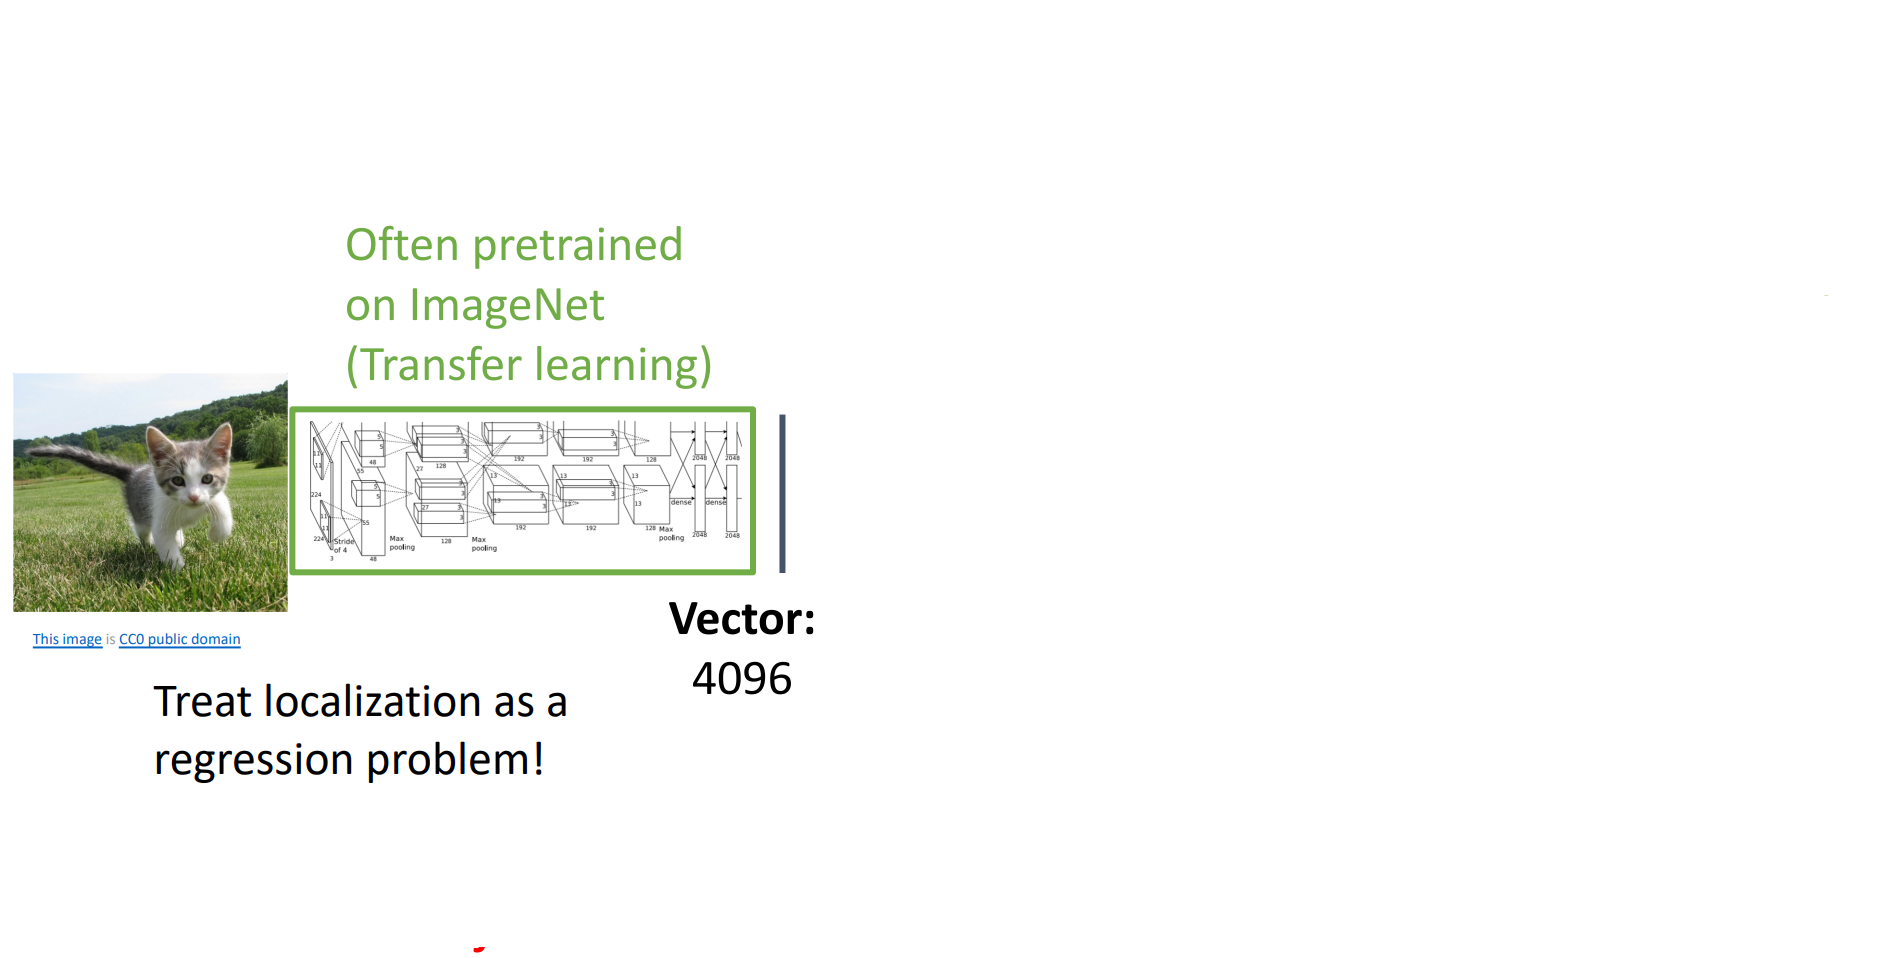
\includegraphics[width=1.0\textwidth,height=0.85\textheight,keepaspectratio]{images/object-detect/object_3.png}
        \caption*{\tiny Source: UMich EECS 498 (2022), Lecture 13: Object Detection, slide 45}
    \end{figure}

\framebreak

    \begin{figure}
        \centering
        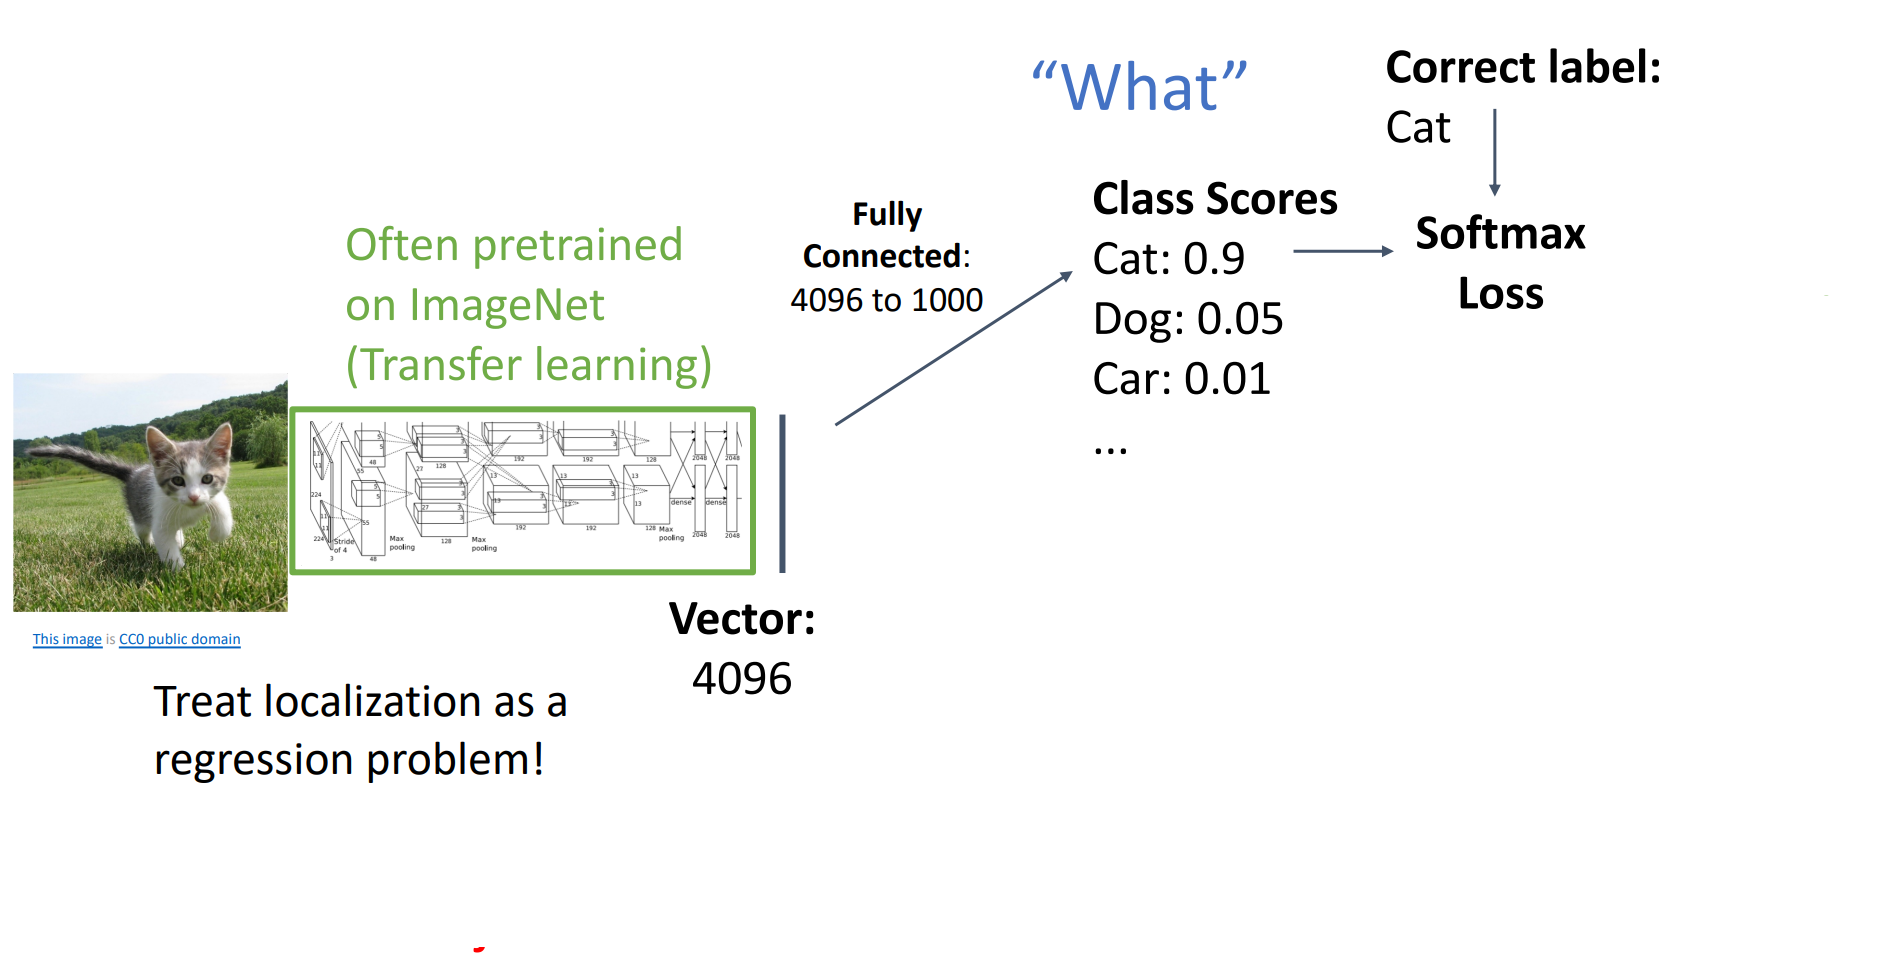
\includegraphics[width=1.0\textwidth,height=0.85\textheight,keepaspectratio]{images/object-detect/object_4.png}
        \caption*{\tiny Source: UMich EECS 498 (2022), Lecture 13: Object Detection, slide 46}
    \end{figure}

\framebreak

    \begin{figure}
        \centering
        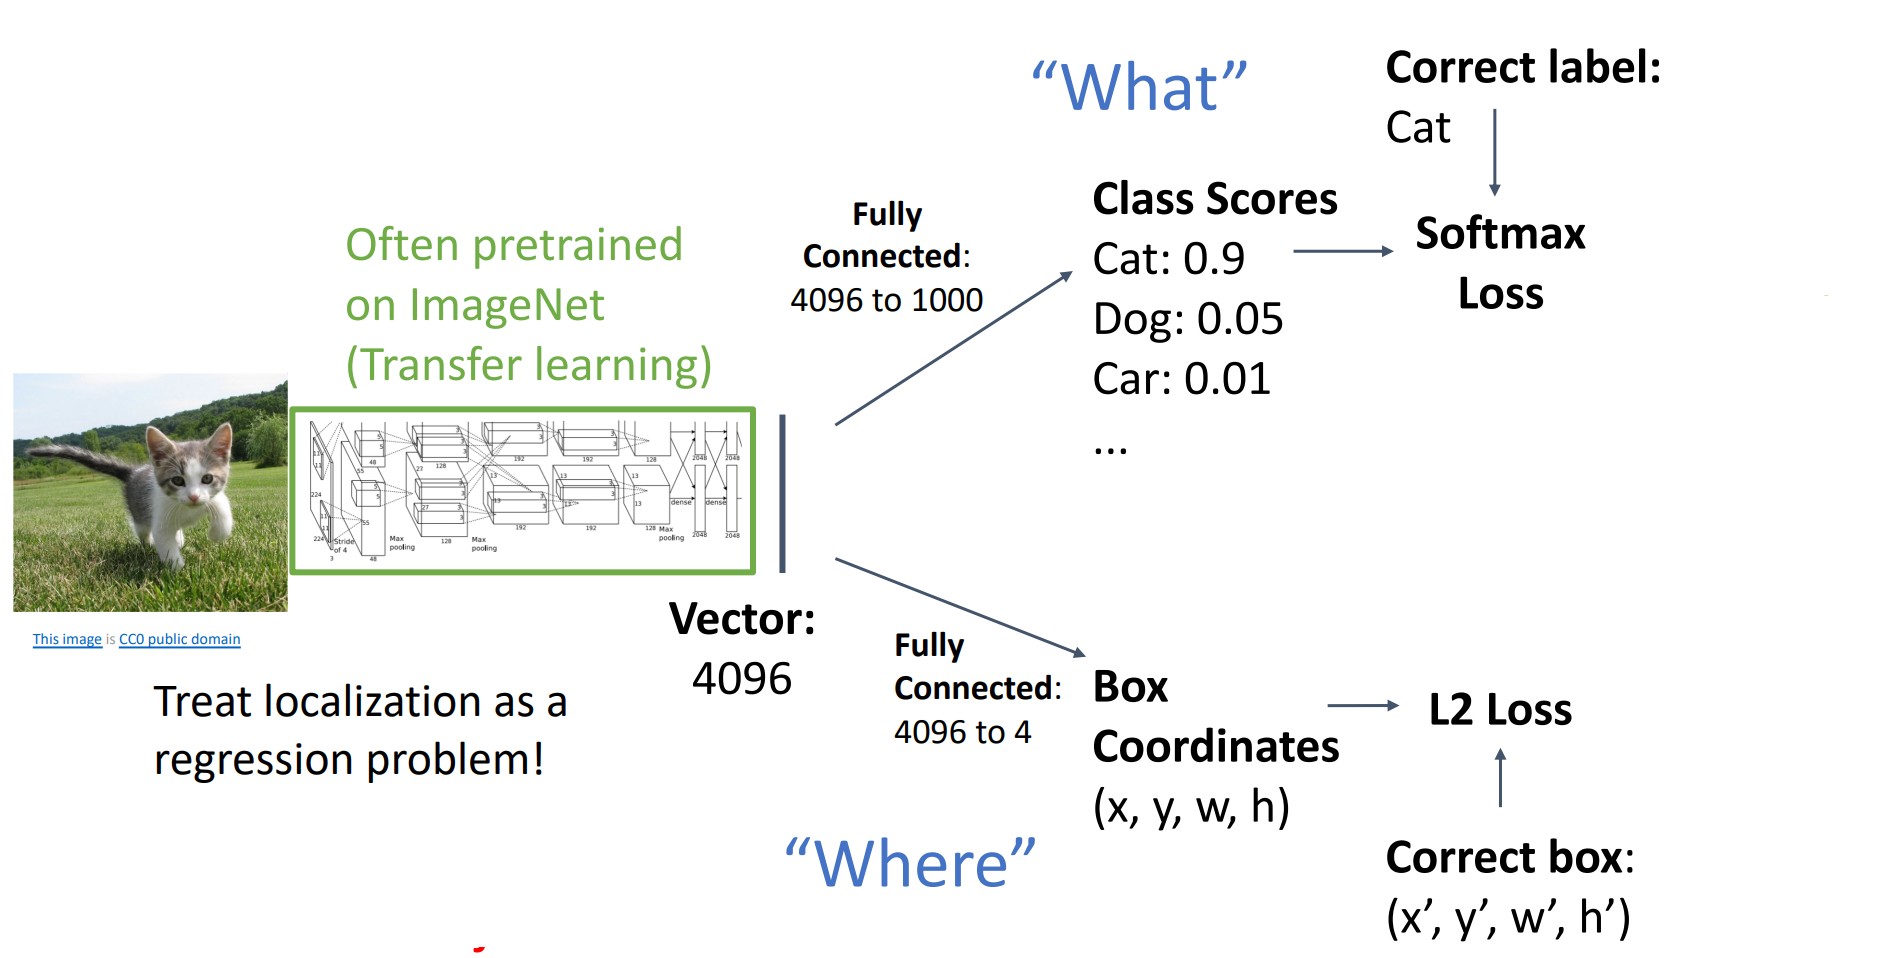
\includegraphics[width=1.0\textwidth,height=0.85\textheight,keepaspectratio]{images/object-detect/object_5.png}
        \caption*{\tiny Source: UMich EECS 498 (2022), Lecture 13: Object Detection, slide 47}
    \end{figure}

\framebreak

    \begin{figure}
        \centering
        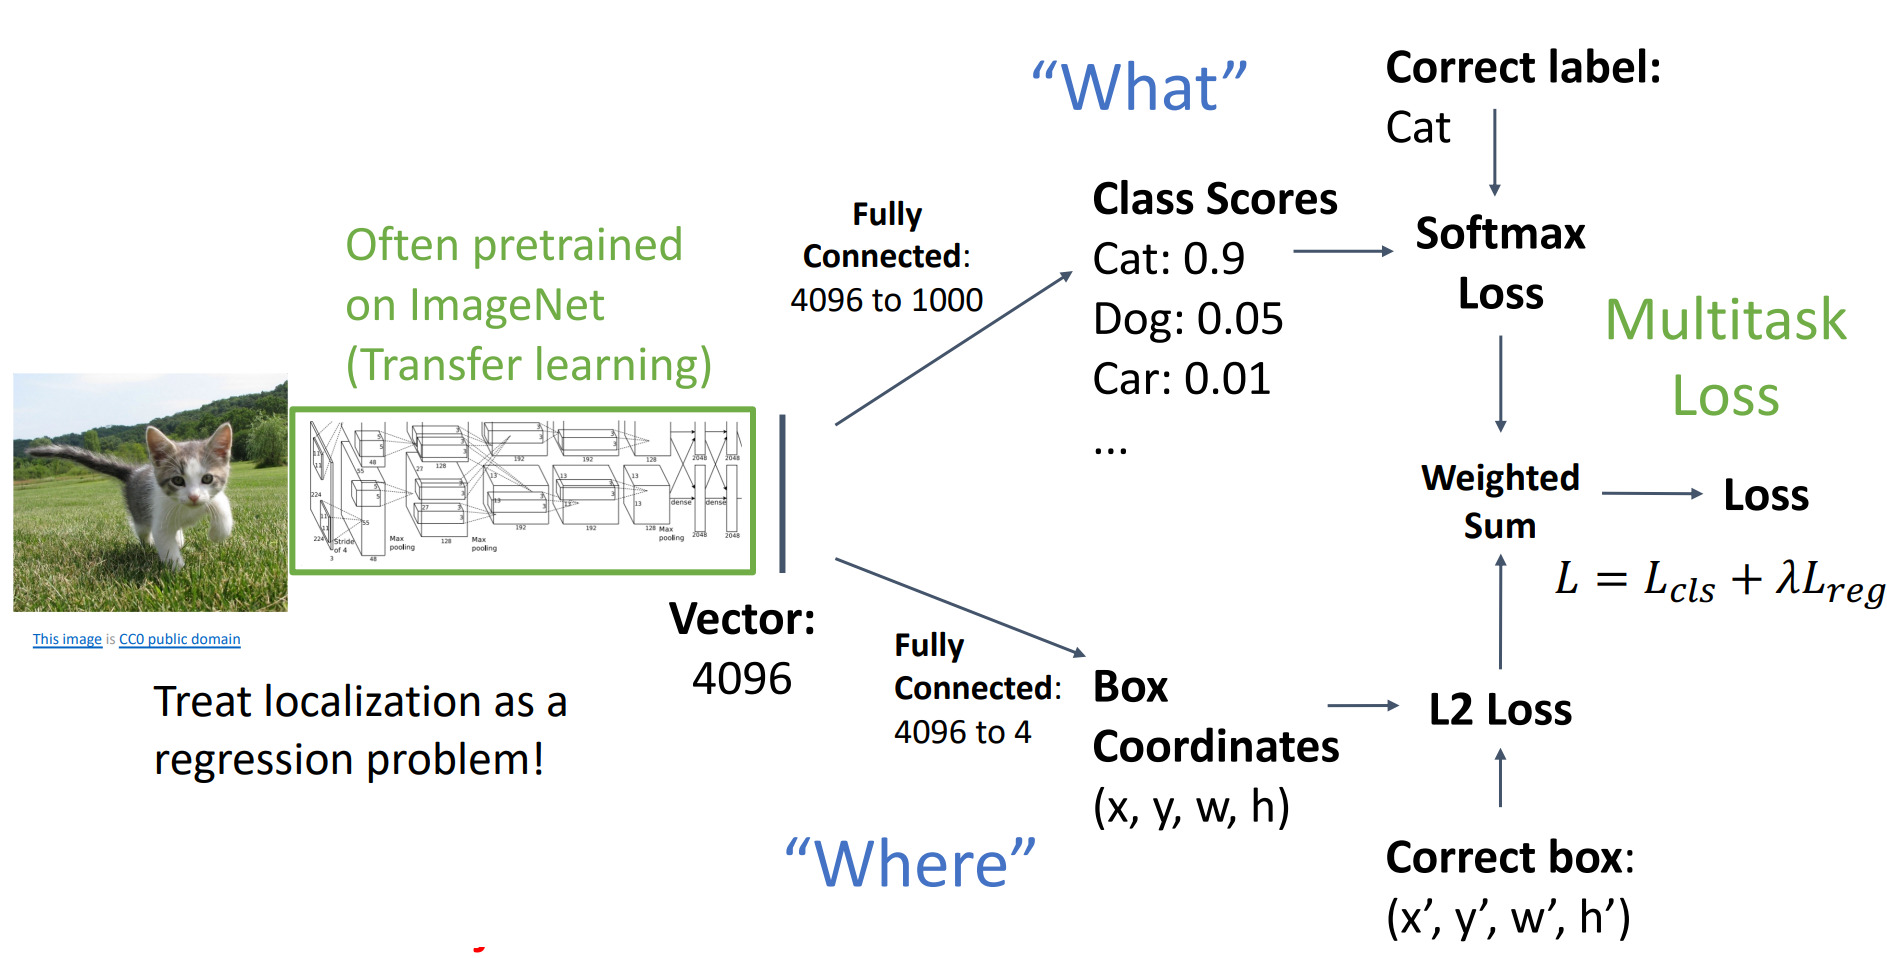
\includegraphics[width=1.0\textwidth,height=0.85\textheight,keepaspectratio]{images/object-detect/object_6.png}
        \caption*{\tiny Source: UMich EECS 498 (2022), Lecture 13: Object Detection, slide 49}
    \end{figure}

\framebreak

    \begin{figure}
        \centering
        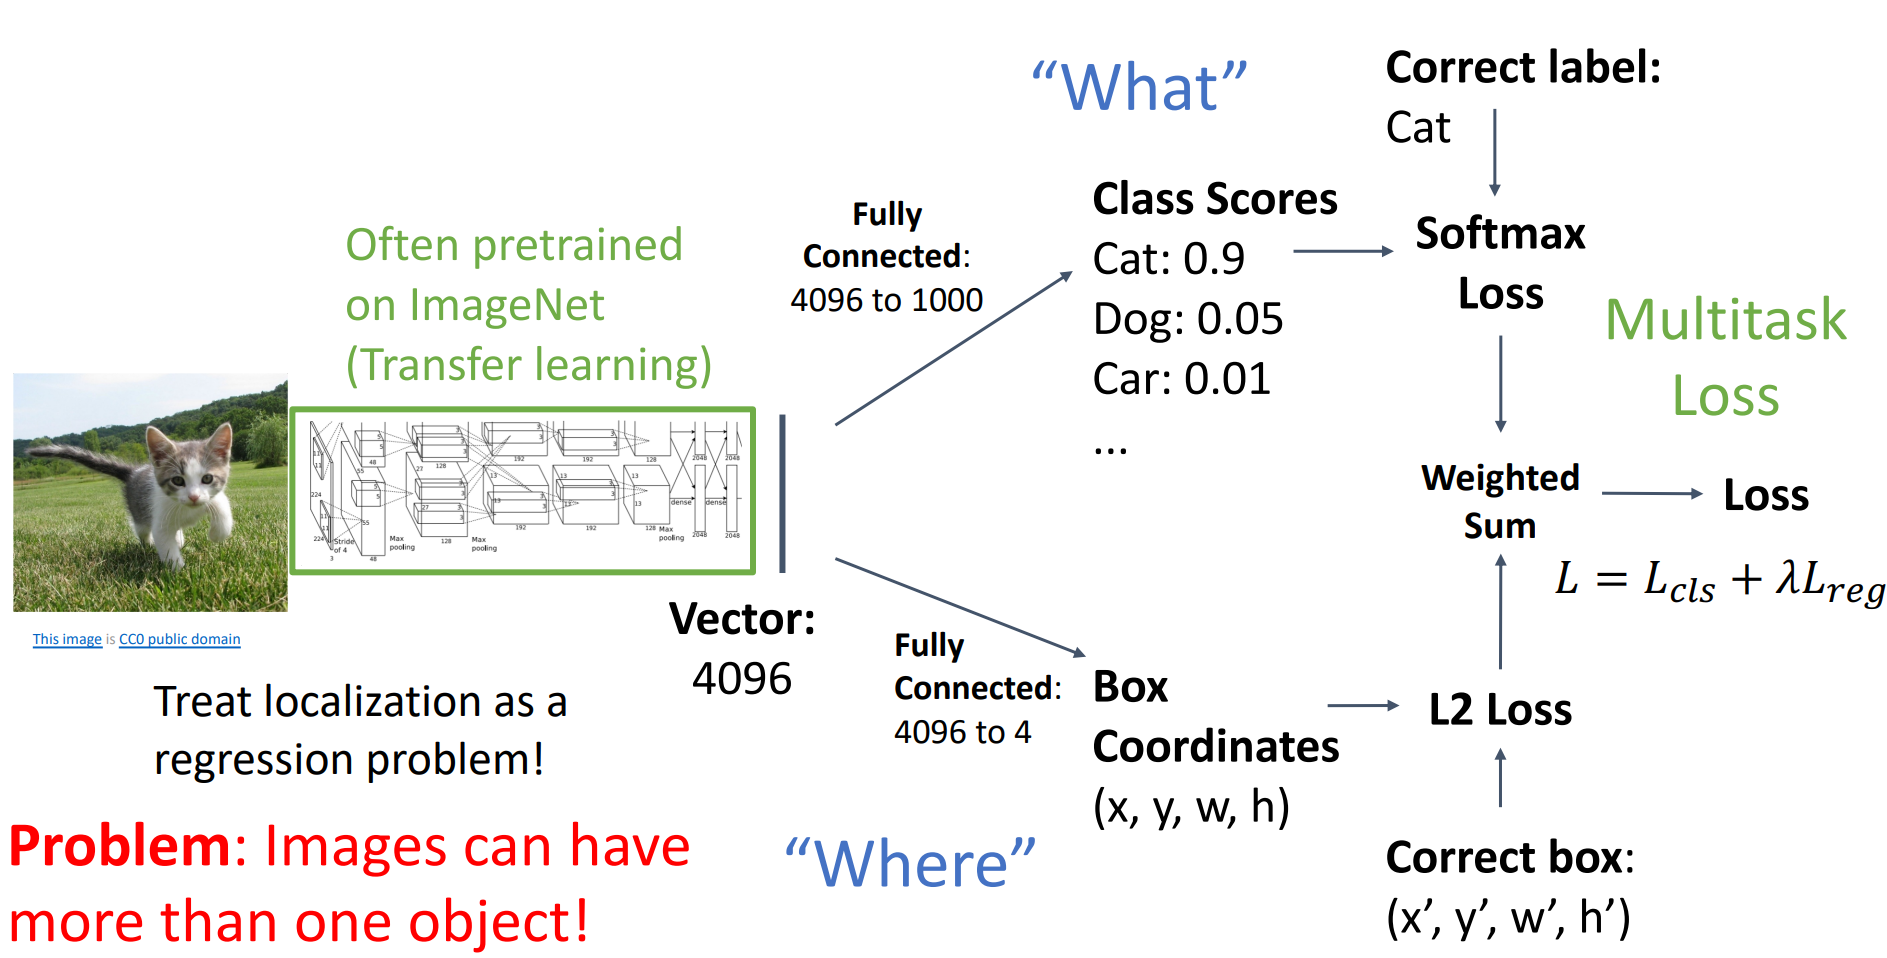
\includegraphics[width=1.0\textwidth,height=0.85\textheight,keepaspectratio]{images/object-detect/object_7.png}
        \caption*{\tiny Source: UMich EECS 498 (2022), Lecture 13: Object Detection, slide 50}
    \end{figure}
    
\end{frame}

